\documentclass[12pt,a4paper]{report}

\usepackage[utf8x]{inputenc}
\usepackage[left=2cm, right=2cm, top=5cm]{geometry}
\usepackage{enumitem}
\usepackage{fontspec}
\usepackage{tikz}
\usepackage{amsmath}
\usetikzlibrary{graphs, shapes, snakes, graphdrawing}

\begin{document}

	\begin{titlepage}
		\centering
		{\scshape\LARGE Universidad Nacional Autónoma de México \par}
		\vspace{1cm}
		{\scshape\Large Computación Distribuida\par}
		\vspace{1.5cm}
		{\huge\bfseries Tarea 5\par}
		\vspace{.5cm}
		{\Large\itshape Edgar Quiroz Castañeda \par}
	    \vspace{.5cm}
		{\Large\itshape Jerónimo Almeida Rodríguez \par}
		\vfill
		 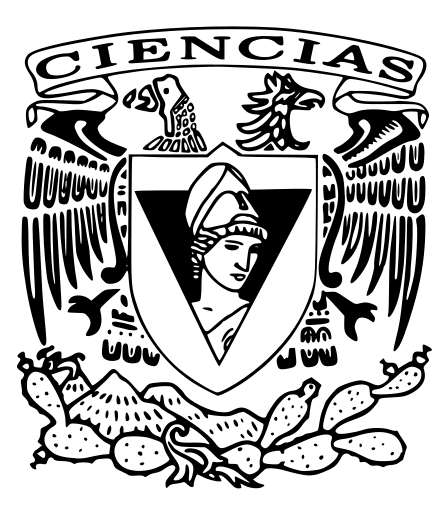
\includegraphics[width=0.5\textwidth]{escudo_f-ciencias.png}
		\vfill

		{\large Jueves 27 de septiembre del 2018 \par}
	\end{titlepage}

	\pagebreak
	\setlength{\voffset}{-0.75in}
	\setlength{\headsep}{5pt}

	\begin{enumerate}
		%Ejercicio 1
		\item {
			Considere la gráfica $G$. Propón retardos y ejecuta el algoritmo PIF con
			$p_1$ como raíz.\\
		}

		%Ejercicio 2
		\item {
			En la Ciudad de México varios puntos de control (nodos) fueron agregados.\\
			Cada uno de estos puntos tiene información de cuantas personas viven
			dentro de cierto diámetro. \\
			Un punto (raíz) de la delegacion Benito Juárez quiere recolectar la
			información de todos los puntos de control. \\
			Escribe un algoritmo para que cada nodo recolecte la información de sus
			hijos para enviarsela al padre sin repetirla.\\

			\begin{algorithmic}[1]
				\State $children \ \leftarrow \emptyset$
				\State $nonChildren \ \leftarrow \emptyset$
				\If{$p_{id}\ =\ root$}
					\State $parent\ \leftarrow\ root$
					\State $send M$ to all neighbors
				\Else
					\State $parent\ \leftarrow\ \bot$
				\EndIf
				\State \upon{receiving $M$ from $p$}
				\Start
					\If{$parent\ =\ \bot$}
						\State $parent\ \leftarrow\ p$
						\State $send M$ to all neighbors except $p$
					\Else
						\State $send nack$ to $p$
					\EndIf
				\End
				\State \upon{receiving $nack$ from $p$}
				\Start
					\State $nonChildren\ \leftarrow\ nonChildren\ \cup\ {p}$
				\End
				\textbf{When} $children\ \cup\ nonChildren\ =\ allMyNeighbours
							\textbf{do}$
				\Start
					\If{$p_{id}\ =\ root$}
						\State END
					\Else
						\State $send\ ack\ to\ parent$
					\EndIf
				\upon{receiving $ack$ from $k$}
				\Start
					\State $add\ k\ to\ children$
				\End
				\End
			\end{algorithmic}
			}

		%Ejercio 3
		\item{
			Demuestre por inducción que en el algoritmo PI, cada nodo $v$ recibe el
			mensaje $M$ por primera vez en a lo más $d(root, v)$.\\

			Por inducción sobre el orden en el que los nodos reciben $M$.\\
			Caso base\\
			Sea $v \in V$ el primer nodo que recibe $M$. Lo recibe en $t(v)$.

			Hipótesisi de inducción.\\
			Todos los nodos que reciben $M$ antes del lugar $k$ cumplen que
			$d(root, v) = t(v)$.\\

			Paso inductivo\\
			Sea $v \in V$ el vértice que recibe $M$ en el lugar $k$.

		}
		%Ejercio 4
		\item{
			Se dice que una digráfica $G = (V, E)$ tiene raiz $r \in V$ y cada
			vértice $v \in V$ es alcanzable desde $r$, es decir, existe un camino
			dirigido alcanzable desde $r$ (un camino dirigido que empieza en $r$ y
			termina en $v$).\\
			Una digráfica $G$ es un  ́arbol dirigido si tiene raíz y la versión no dirigida
			de $G$ es un árbol. Demuestra el siguiente teorema:\\

			\textbf{Teorema 1}\\
			Sea G una digráfica. Las siguientes condiciones son equivalentes
			\begin{enumerate} [label = \alph*)]
				\item {
					$G$ es un árbol dirigido.\\
				}
				\item {
					$G$ tiene una raíz desde la cual hay un único camino dirigido a
					vértice.\\
				}

				\item{
					$G$ tiene una raíz $r$ para la cual $\delta(r)_{in} = 0$, y para cualquier
					otro vértice $v$, $\delta_{in}(v) = 1$.\\
				}

				\item{
					$G$ tiene una raíz $r$ y el quitar cualquier arista interumpe la
					condición.\\
				}
				\item{
					La versión no dirigida de $G$ es conexa y $G$ tiene un vértice $r$ para
					el cual $\delta_{in}(t) = 0$ mientras que para cualquier otro vértice
					$v$ $\delta(v)_{in} = 1$.\\
				}
			\end{enumerate}

			$a \implies b$\\
			Sea $G$ un árbol dirigido. Por definición, significa que tiene una raíz,
			esto es un vértice desde el cuál hay un camino a cualquier otro vértice de
			$G$.\\
			Sólo falta ver que ese camino es único.\\

			Primero, notemos que esos camino son trayectorias, pues si uno de estos
			caminos, dígamos $c = (r = v_1, ..., v_n)$ tuviera un vértice repetido,
			digamos $v_i = v_j, i < j$, entonces $c' = (r = v_1, ..., v_i = v_j, ... v_n)$
			sería un cliclo en la versión no dirigida de $G$, por lo que la versión
			no dirigida de $G$ no sería un árbol.\\

			Luego, tomemos dos de estas trayectorias $c_1 = (r = v_1, ..., v_n = u)$ y
			$c_2 = (r = w_1, ..., w_m = u)$ y supongamos que son diferentes.\\
			Sea $v_i = w_j \in V$ el primer vértice no raíz que hay en común entre
			$c_1$ y $c_2$, cuya existencia se puede garantizar porque en el caso
			extremo este vértice es $u$.\\
			Entonces, en la versión no dirigida de $G$, consideremos el camino
			$c_3 = (r = v_1, v_2, ..., v_i = w_j, w_{j-1}, ..., w_2, w_1 = r)$.\\
			Cómo los $v_k$ provienen de una trayectoria, entonces no se repiten entre
			sí, al igual que los $w_l$.\\
			Además, como $v_i = w_j$ es el primer vértice en común entre las
			trayectorias originales, entonces los $v_k$ y  los $w_l$ no tienen ningún
			otro vértice en común.
			Entonces $c_3$ es una trayectoria, y comienza  y termina en el mismo
			vertice, por lo que es un ciclo.\\
			Entonces, la versión no dirigida de $G$ no es un árbol, lo cuál no es
			posible. Esta contradicción surge de suponer que $c_1$ y $c_2$ eran
			diferentes. Entonces, cualesquiera dos caminos entre la raiz y un mismo
			vértice son en realidad el mismo.\\
			Entoces el camino dirigido entre la raíz y cualquier vértice es único.\\

			$b \implies c$\\
			Sea $G$ una gráfica dirigida con una raíz $r$ y cuyos caminos entre la raíz y
			cualquier otro vértice son únicos.\\
			Veamos que $\delta(r)_{in} = 0$. Por contradicción, supongamos que
			$\delta(r)_{in} < 0$. Entonces sea $v \in N^+(r)$. Como $r$ es raíz,
			entonces existe un camino, que ya sabemos es trayectoria,
			$c = (r = v_1, ..., v)$. Entonces, $c' = (r = v_1, ..., v, r)$ es un
			ciclo en la versión no dirigida de $G$, pero esta debe de er un árbol.
			Entonces $\delta(r)_{in} = 0$.\\
			Luego, veamos cuál es el grado interior de los demás vértices.
			Sea $w \in V$. Como hay un camino $c_1 = (r = w_1, ..., w_n = w)$,
			entonces al menos un vértice $w_{n-1}$ incide en $w$, por lo que
			$\delta(w)_{in} \geq 1$.\\
			Luego, supongamos que $\delta(w)_{in} > 1$. Entonces sean
			 $u_1, u_2 \in N^+(w), u_1 \neq u_2$.\\
			Como $r$ es raíz, entonces existen caminos únicos $s_1 = (r = x_1, ..., x_n = u_1)$
			y $s_2 = (r = y_1, ..., y_n = u_2)$.\\
			Tanto $s_1$ como  $s_2$ inciden es $w$, entonces
			$s_1 = (r = x_1, ..., x_n = u_1, w)$ $s_2 = (r = y_1, ..., y_n = u_2, w)$
			son dos caminos de la raiz a $w$ diferentes, pues al menos $x_n = u_1 \neq y_n = u_2$.
			Pero los caminos desde la raíz son únicos. Esta contradicción surge de
			asumir que $\delta(w)_{in} > 1$.\\
			Por lo tanto, $\delta(w)_{in} = 1$.\\

			$c \implies d$
			Sea $G$ una gráfica que tiene una raíz $r$ para la cual $\delta(r)_{in} = 0$,
			y para cualquier otro vértice  $v \in V$, $\delta_{in}(v) = 1$.
			Cómo $G$ tiene raíz, sólo falta demostrar que $G-\{e\}, e \in E$ no tiene
			raíz.
			Sea $e = (v, w) \in E$.
		}
	\end{enumerate}
\end{document}
